\chapter{Proposed system}

To be able to locate an object with no previous knowledge of the object (such
as its size, color and so on), two views of the same object are needed. The
views can be obtained by one moving camera or by multiple cameras. In this
thesis, we take a closer look at the second approach.

We propose a system with two cameras, connected via USB to a computer.
Two cameras provide enough information for object localization and make the
project usable also on low-budget. The placement of the cameras is important,
but no precise alignment is required. The cameras should share a significant part
of the view (see an example of the setup in the figure \ref{fig:camera-setup}).

\begin{figure}
	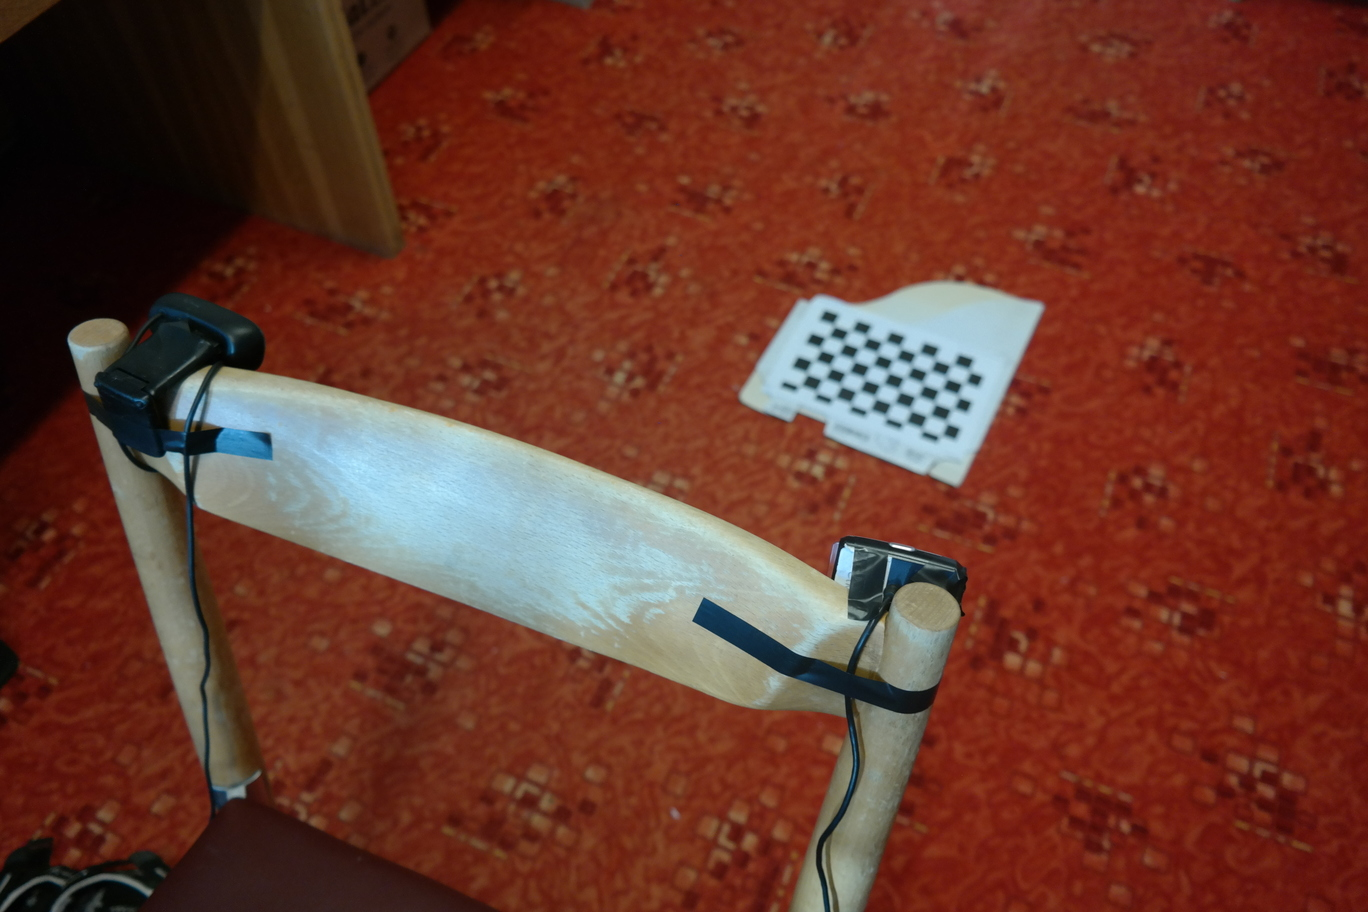
\includegraphics[width=\linewidth]{img/camera-positions.jpg}
	\caption{Example of camera setup}
	\label{fig:camera-setup}
\end{figure}

Our solution is able to estimate the positions of the cameras (relatively to
each other) using an automated calibration process. After calibration, the user
marks an object to be tracked in the view of each camera. The estimated
position of the cameras and the object is then displayed. We describe each step
of the process in the following chapters.

\section{Tools}

For the computer vision task, we use an \emph{OpenCV} library. OpenCV is an open
source computer vision library with many algorithms implemented (for example
calibration, triangulation, and so on). We use trackers which are now available
only in the \emph{contribute} version. For more information and examples of usage
visit their webpage\footnote{\url{https://opencv.org/}}.

To provide a comparison of trackers, we also include one tracker from
\emph{Dlib}\footnote{\url{http://dlib.net/}} library. It is also open source
and an interface for the Python is provided.  Since this library focus is on
machine learning, it does not contain as many functions for computer vision
as the OpenCV library yet.

\section{Notations}

The following section describes some procedures using math notion. To avoid
ambiguity we provide the overview of the used notation here.

\subsubsection*{Vector}
A word \emph{vector} denotes a column vector in a shape of $n\times1$.

\subsubsection*{Block matrix}
A matrix operation $W = (A|B)$, where $A$ is a matrix $m \times n$ and B is a
matrix $m \times p$, creates matrix $W$, where first $n$ columns are the entries from
matrix $A$ and last columns consist of the columns of the matrix $B$.
Example:

\[
A = \begin{pmatrix}
        1 & 2 \\
        3 & 4
\end{pmatrix},
B = \begin{pmatrix}
5 \\
6
\end{pmatrix},
(A|B) = \begin{pmatrix}
        1 & 2 & 5 \\
        3 & 4 & 6
\end{pmatrix}
\]

\subsubsection*{Homogenous coordinates}

In computer vision homogenous coordinates are used frequently instead of
Cartesian coordinates.  These coordinates have one element added. This elemnt
is scaling factor. As an example, vector $(2x, 2y, 2z, 2)^T$ represents same
point as $(x, y, z, 1)^T$ in homogenous coordinates. The same point is equal to
$(x, y, z)^T$ in Cartesian coordinates. Unlike the Cartesian coordinates, a
single point can be represented by infinitely many homogenous coordinates.

Similarly it works for coordinates in any n-dimensional space. In conversion
from Cartesian to homogenous coordinates we simply add new elemnt at the end
equal to one. In the opposite direction, we divide first $n-1$ values by the
$n$th.

In homogenous coordinates the origin is ommited. Homogenous coordinates provide
us also a way how to represent point in the infinity by finite coordinates.
These points in the infinity are represented with the scale factor equal to 0.

This coordinates representation is tightly bounded to a projective plane, on
which the mathematical theory behind is based. For us is just important to know
how to convert them to Cartesian coodinates and that algorithms for computer
vision often use them.
